% !TEX root = ../main.tex
\begin{center}
{\large {\bf Collaboration Plan}} \\
\end{center}
The proposed project team consists of two PIs (Yanyong Zhang and Lin Zhong), one senior personnel (XYZ), one postdoctoral researcher, and three graduate students. 

\subsection*{Team Expertise}
The two PIs and the senior personnel bring complementary expertise for the proposed research.

{\bf PI Yanyong Zhong}  


{\bf PI Lin Zhong} is a leading expert in mobile computing, including energy optimization and computer vision applications. His work has won best paper awards from ACM MobileHCI 2007~\cite{rahmati2007mobilehci}, IEEE PerCom 2009~\cite{liu2009percom}, ACM MobiSys 2011~\cite{dong2011mobisysa}, ACM MobiSys 2013~\cite{likamwa2013mobisysa}, ACM ASPLOS 2014~\cite{lin2014asplos}, and ACM MobiSys 2014~\cite{amirisani2014mobisys}.  In recent years, he has investigated operating system support for programming heterogeneous mobile SoC~\cite{lin2012asplos,lin2012hotpower,lin2014asplos}. This endeavor has not only led to early results for the proposed research but also led him and his team to realize the importance of programming system support for solving the problem. 

{\bf Senior Personnel XYZ} is the leading research scientist in 

{\bf Postdoctoral Researcher} support is included in the project budget. For this position, we will target at recruiting expertise in XYZ

\subsection*{Collaboration and Task Management}

PI Zhang will oversee the project and ensure its integration and success. 

\begin{figure}
    \centering
    \begin{minipage}[5cm]{0.44\textwidth}
    \centering
 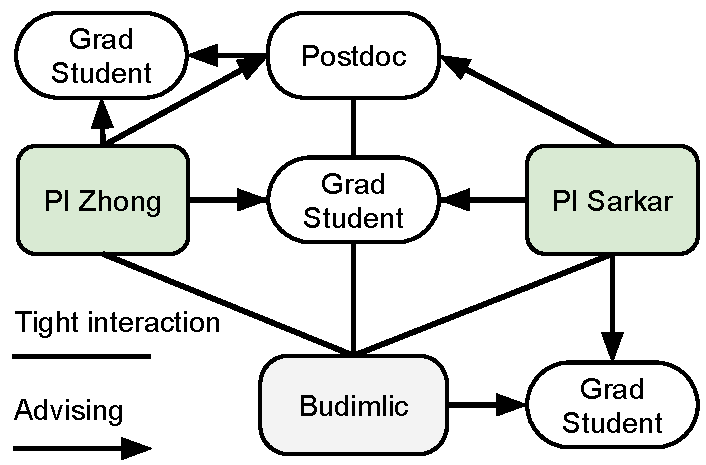
\includegraphics[height=0.17\textheight]{figs/collaboration}
%    \caption{\textit{Timeline for the proposed project}}
%    \label{fig:timeline}
    \end{minipage}
\hspace{+2mm}
    \begin{minipage}[5cm]{0.46\textwidth}    \centering
 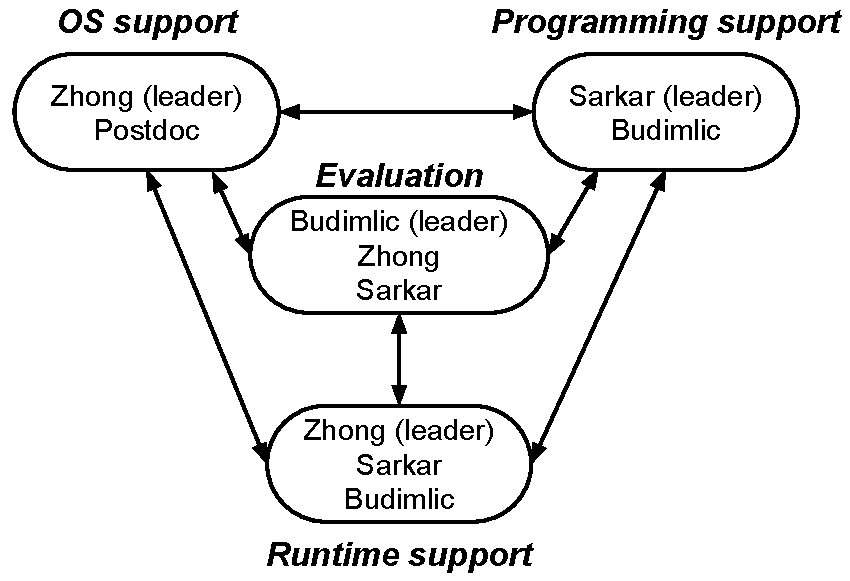
\includegraphics[height=0.18\textheight]{figs/taskmanagement}
    \end{minipage}
 \caption{\textit{(\emph{Left}) Graph of personnel and major interactions; and (\emph{Right}) Project task management with lead PI and participating PIs for each major research thrust.}}
    \label{fig:collaboration}
\end{figure}

While the two PIs have not had a joint NSF grant, they have already built a collaborative relationship due to their mutual interests in each other's research. 

\subsection*{Project Timeline\label{sec:management}}
The proposed project will be accomplished in four years. Figure~\ref{fig:timeline} presents the timeline for the major activities of the project. We emphasize the iterative nature of the three research thrusts and the evaluation plan because findings from one thrust are likely to change the course of another.  The education and outreach plan will be carried out through the four years.

%\begin{wrapfigure}{r}{0.75\textwidth}
%    \centering
% 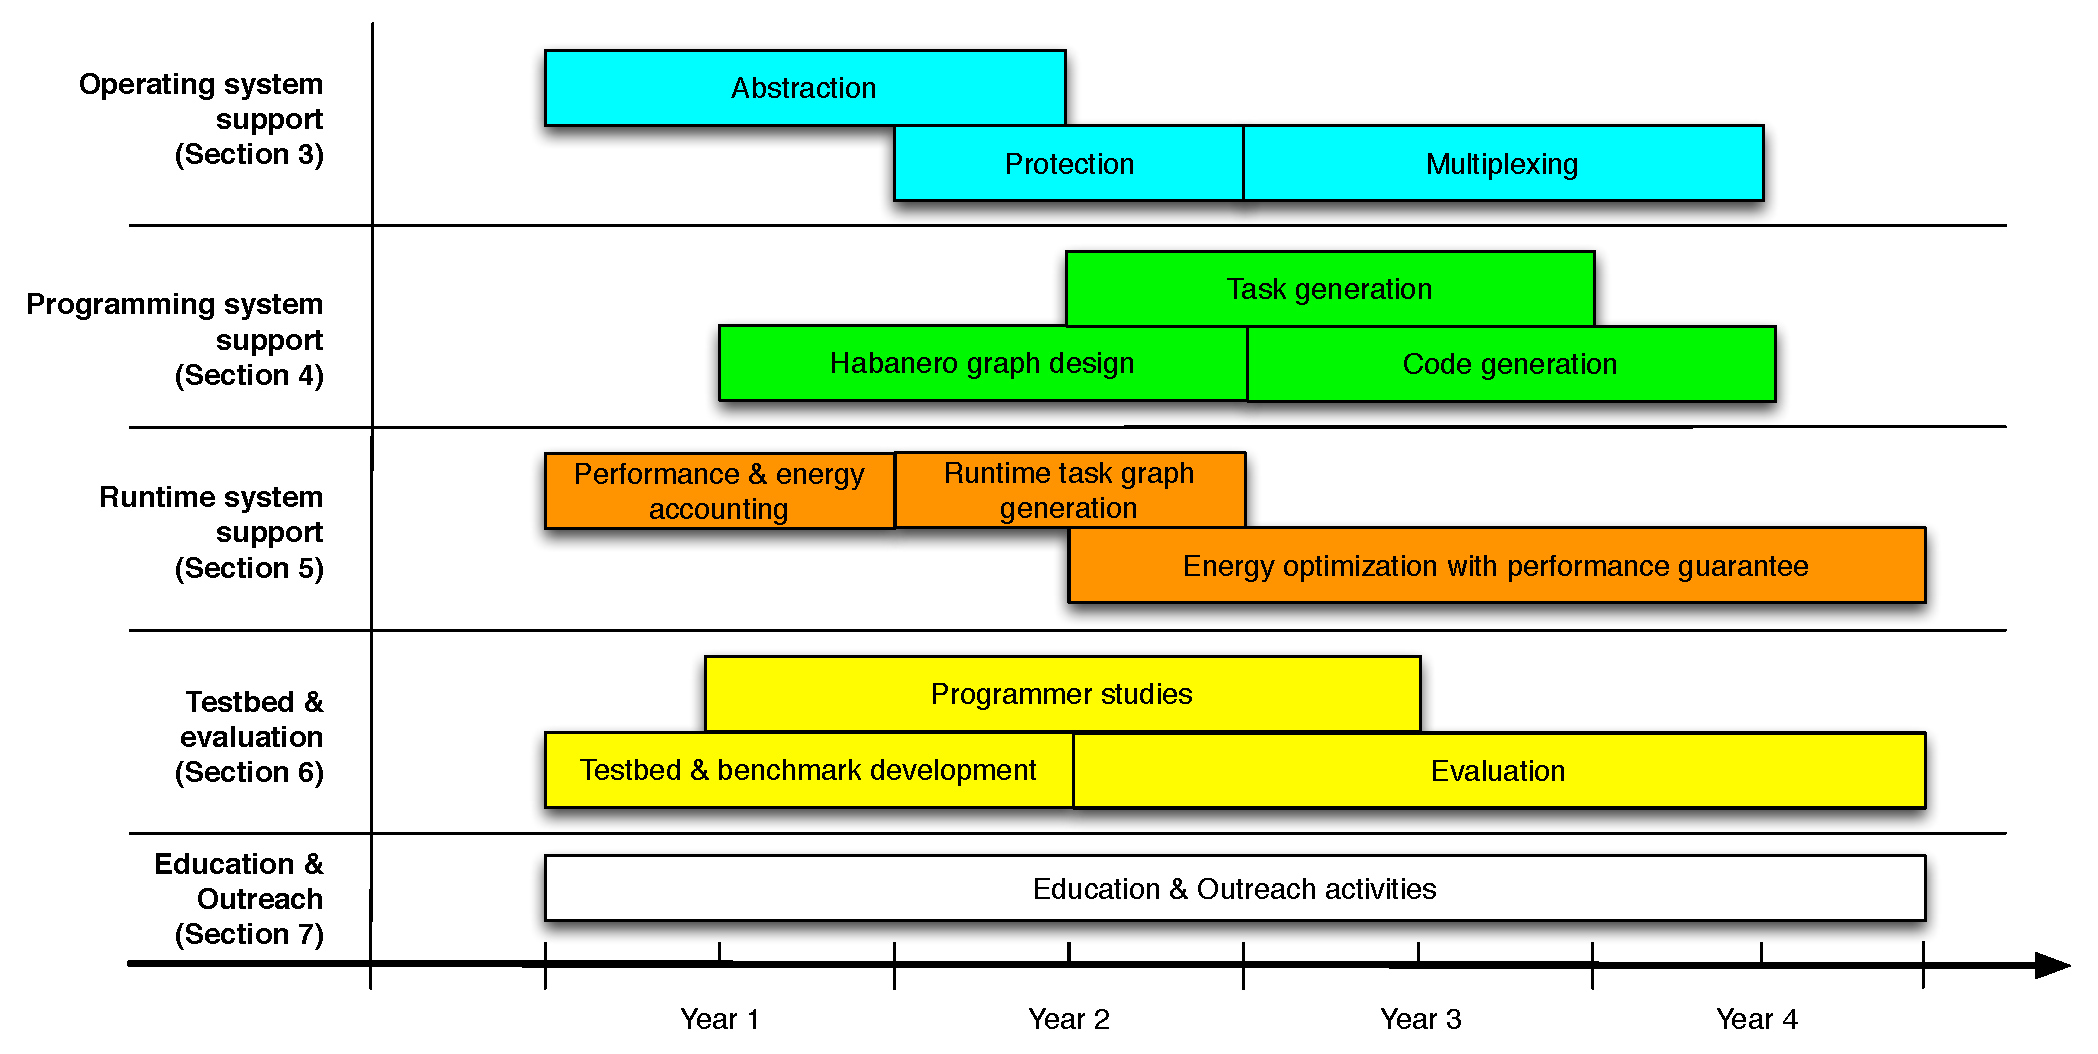
\includegraphics[width=0.75\textwidth]{figs/task-timeline}
%    \caption{\textit{Timeline for the proposed project}}
%    \label{fig:timeline}
%\end{wrapfigure}

\begin{figure}
    \centering
 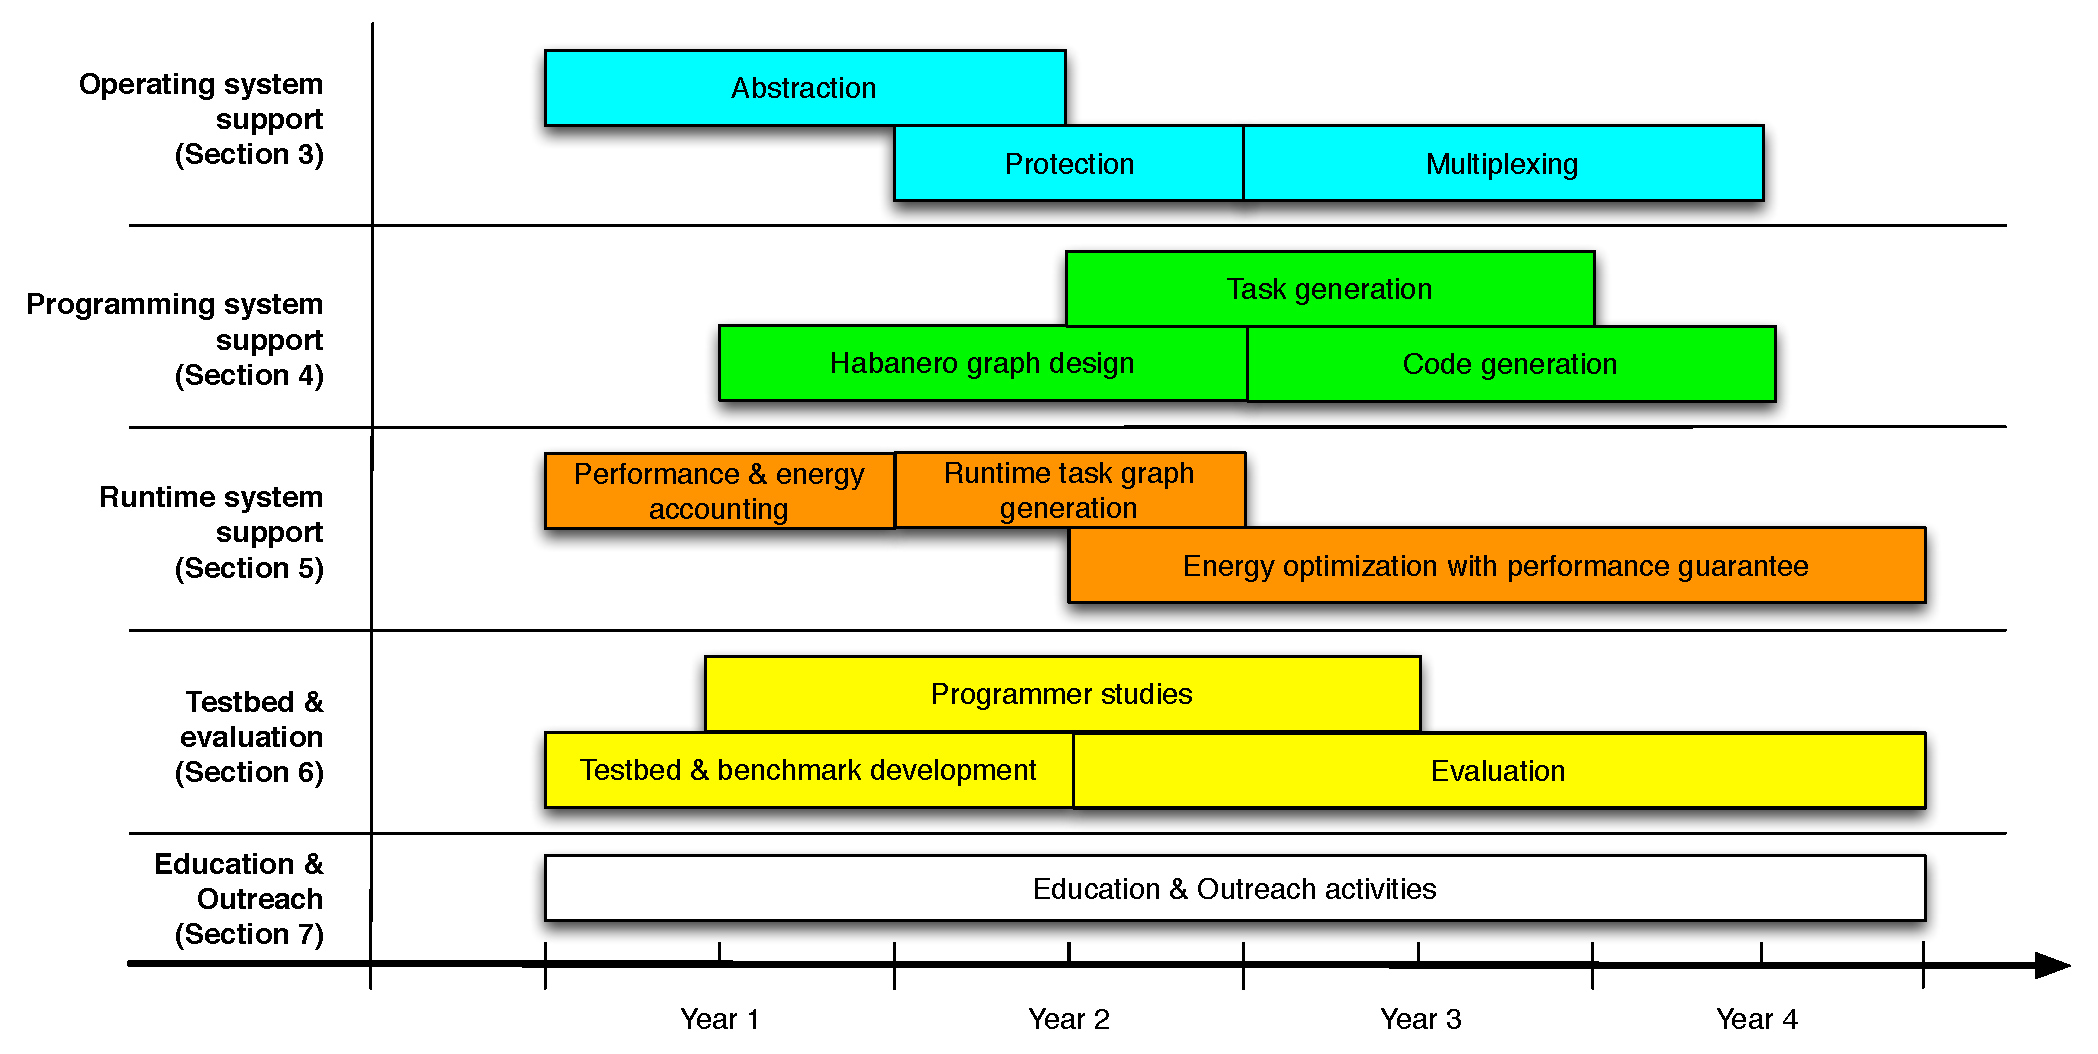
\includegraphics[width=0.75\textwidth]{figs/task-timeline}
    \caption{\textit{Timeline for the proposed project}}
    \label{fig:timeline}
\end{figure}

\subsection*{Coordination Mechanisms}
All members of the project team and their laboratories are located in the same building (Duncan Hall) on Rice campus, which greatly facilitates the project coordination. In addition, we will employ the following measures to ensure timely coordination of all research thrusts. (\textit{i}) First, we will use \emph{weekly team meeting} to foster face-to-face discussion and timely exchange of ideas. (\textit{ii}) Second, we will utilize  a \emph{Web-based internal collaboration system} called \emph{OWL-Space}~\cite{owlspace} to foster on-line discussion. Team members will also use this web system to provide weekly updates of their research and document milestones in their development.  (\textit{iii}) Third, we will use a \emph{Web-based public collaboration system (Wiki)} to host software and documentation releases to the public. It will also allow the public to provide feedbacks and foster a user community of the tools and software resulting from the proposed project. 
